\newpage
\section{NVIC}
    \subsection{Wir wird er verwendet}
        Beim Programmieren des STM muss der Vector Table beschrieben werden mit einem Assembler File und Linker Skript, diese werden von der Cube IDE erstellt.\\
        Im Vector Table sind alle Interrupts mit dem entsprechenden Funktionnamen für das Programm hinterlegt.
        Im NVIC\_ISER Register können die Interrupts durch ihre Interrupt Position aktiviert werden.\\\\
        Die IRQ\_Handler Positionen werden beim programmieren des uC in den Flash geschrieben. 

        \begin{figure}[!htb]
            \centering
            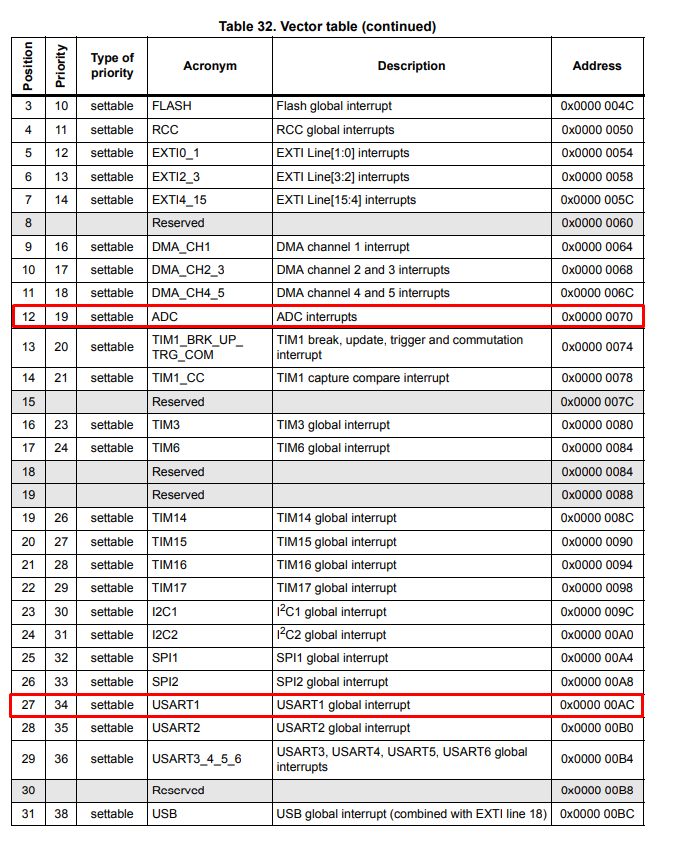
\includegraphics[scale=0.65]{NVIC-Vector-Table.png}
            \caption{NVIC-Vector-Table}
            \label{caption:ANVIC-Vector-Table}
        \end{figure}

\newpage
        \begin{figure}[!htb]
            \centering
            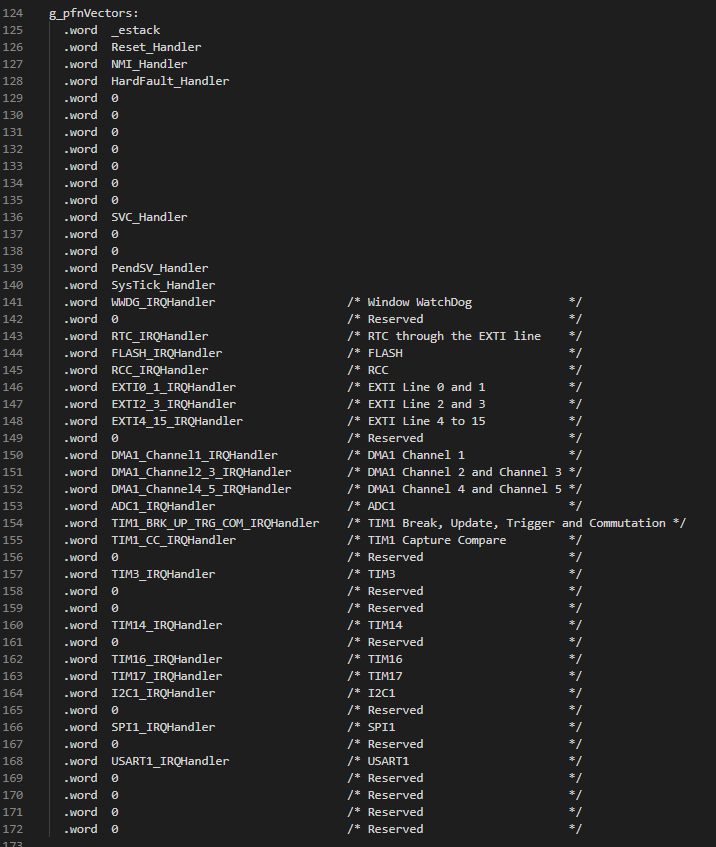
\includegraphics[width=\linewidth]{Ausschnit-Assembler-File.png}
            \caption{Ausschnit-Assembler-File}
            \label{caption:Ausschnit-Assembler-File}
        \end{figure}
\newpage
        \begin{figure}[!htb]
            \centering
            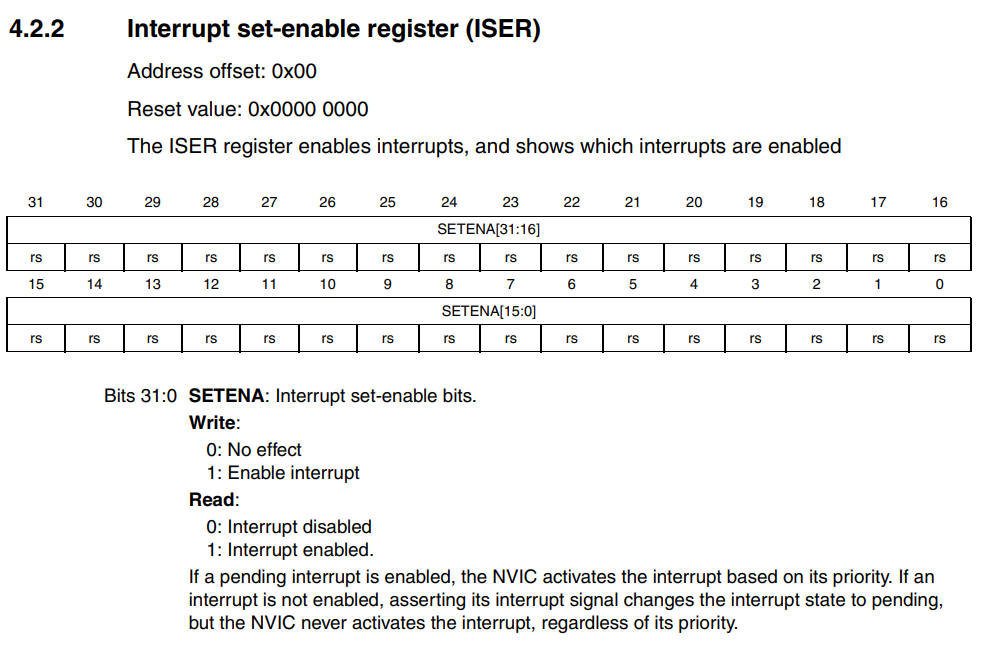
\includegraphics[width=\linewidth]{NVIC-ISER-Register.png}
            \caption{NVIC-ISER-Register}
            \label{caption:NVIC-ISER-Register}
        \end{figure}
        
    \subsection{NVIC-Code}
        \begin{lstlisting}[language=C, style=CStyle, caption=NVIC-enable-interrupts, captionpos=b, label=NVIC-enable-interrupts]
void NVIC_enable_interrupts(void)
{
    uint32_t* nvic_iser =  NVIC_ISER;
    uint32_t reg_content;
    reg_content = *nvic_iser;
    reg_content |= 0x08001000;
    *nvic_iser = reg_content;
}
        \end{lstlisting}
